\section{Security Analysis of Suffix Proofs}

\subsection{Superchain Quality \& Suppression Attacks}

As explained earlier, every $\mu-$superblock represents $2^\mu$ 0-level blocks in expectation, or $\mu-$ superblocks occur approximately once every $2^\mu$ blocks. Put in another way, each $\mu-$superchain $\chain$ has an underlying chain of length $2^\mu \lvert \chain \rvert$ in expectation. This chain property is referred ``superchain quality'' or ``goodness'' of the chain. A formal definition can be found in~\cite{nipopows}.

It's easy to see that the goodness property holds with overwhelming probability for chains generated in optimistic environments, i.e. if no adversary tries to violate the superblock distribution. However, an adversary can harm superchain quality by performing suppression attack to one or more superblock level. In order to see this consider an adversary $\mathcal{A}$ who breaks the superchain quality of an honestly adopted chain $\chain_B$ at level $\mu$ as follows. $\mathcal{A}$ starts playing after $\lvert \chain_B \rvert \geq 2$ and inspects the appended blocks at every round. If $\text{level}(\chain_B[-1]) < \mu$, then $\mathcal{A}$ remains idle. However, if $\text{level}(\chain_B[-1]) \geq \mu$ then $\mathcal{A}$ tries to mine an adversarial block $b$ on top of $\chain_B[-2]$. If successful she tries to mine one more block $b'$ on top of $b$. If successful again, she broadcasts $b, b'$. Now, with non-negligible probability~\cite{nipopows} the adversary generates $b, b'$ soon enough, so that honest party $B$ adopts the chain containing them. This would mean that the last $\mu$-superblock is successfully supressed. In any case, the adversary continues her attack by restarting her strategy, inspecting the level of $\chain[-1]$ and acting accordingly. An execution of this attack is illustrated in Figure~\ref{fig:superquality_attack}. It's abvious that several honest $\mu$-superblocks are successfully suppressed causing harm to the superchain quality. 

\begin{figure}[h!]
	\begin{center}
		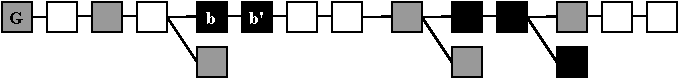
\includegraphics[width=0.7\columnwidth]{figures/superquality_attack.pdf}
	\end{center}
	\caption{Superquality attack. The adversary performs a selfisj mining~\cite{selfish} attack (black blocks) whenever an honest $\mu$-superblock (grey) is mined. The attack affects the distribution of $\mu$-superblocks in the honest chain~\cite{nipopows}.}
	\label{fig:superquality_attack}
\end{figure}

In parallel to performing this attack the adversary may also maintain a fork chain. Assuming honest majority, the adversary's fork chain will be shorter than the honest parties' chain at 0-level. However, the adversary's $\mu$-superchain might be longer than that of the honest parties' because of the superquality attack on the honest chain. Thus the adversary may successfully fool the verifier to favor her proof. As formally proven in~\cite{nipopows} the adversary can produce a winning suffix proof for her fork chain with non-negligible probability.

The modified proof construction is given in Algorithm~\ref{alg:goodness_aware_suffix_prover_soft_fork} and allows the prover to take superchain goodness into account. More in detail, at each step the prover checks the $\mu$-superblock distribution quality in the subchain $\alpha$ before moving on to the lower superchain level. If goodness is indeed maintained at the current level then the prover regularly covers the span of the last m $\mu$-level blocks with blocks of level $\mu-1$. Otherwise, if goodness is violated for level $\mu$ then the prover completely ignores this level and tries to span the whole range of subchain $\alpha$ with blocks of the lower level $\mu - 1$.

\begin{algorithm}[h]
		\caption{\label{alg:goodness_aware_suffix_prover_soft_fork}The \textit{goodness aware} Suffix Prover for the superblock NIPoPoW protocol~\cite{nipopows}}
		\begin{algorithmic}[1]
				\Function{\sf Prove$_{m,k}$}{$\chain$}
					\Let{B}{\chain[0]}
					\For{$\mu = \lvert \chain[-k].\textsf{interlink} \rvert$ down to $0$}
						\Let{\alpha}{\chain[{:}-k]\{B{:}\}\upchain^\mu}
                        \Let{\pi}{\pi \cup \alpha}
                        \If{$\text{good}_m (\chain, \alpha, \mu)$}
						    \Let{B}{\alpha[-m]}
                        \EndIf
					\EndFor
					\Let{\chi}{\chain[-k{:}]}
					\State\Return$\pi\chi$
				\EndFunction
		\end{algorithmic}
\end{algorithm}

\subimport{./}{security_proof_suffix.tex} 